\documentclass[
      aspectratio=169,
        12pt,
    ]{beamer}

% ------------------------------------ font
\usefonttheme[onlymath]{serif}
\usepackage[T1]{fontenc}
\usepackage{textcomp}
\usepackage[scale = 1.0]{tgheros} %Sans serif
\usepackage[scaled]{beramono}
\usepackage{luatexja-otf}
\usepackage[match, deluxe, expert, noto-otf]{luatexja-preset}
\renewcommand{\kanjifamilydefault}{\gtdefault}

% ------------------------------------ math packages
\usepackage{amsmath,amssymb}
\usepackage{siunitx}

% ------------------------------------ comment out package
\usepackage{comment}

% ------------------------------------ tables
\usepackage{longtable, booktabs, array}
\usepackage{threeparttable, threeparttablex, multirow}
\newcolumntype{d}{S[input-symbols = ()]}

% ------------------------------------ figures
\usepackage{graphics, graphicx}
\makeatletter
\def\maxwidth{\ifdim\Gin@nat@width>\linewidth\linewidth\else\Gin@nat@width\fi}
\def\maxheight{\ifdim\Gin@nat@height>\textheight\textheight\else\Gin@nat@height\fi}
\makeatother
% Scale images if necessary, so that they will not overflow the page
% margins by default, and it is still possible to overwrite the defaults
% using explicit options in \includegraphics[width, height, ...]{}
\setkeys{Gin}{width=\maxwidth,height=\maxheight,keepaspectratio}

\usepackage{tikz}
\usetikzlibrary{backgrounds}

% ------------------------------------ other packages (header-includes)

% ------------------------------------ Slide Designs
\definecolor{DarkBlue}{rgb}{0.05, 0.15, 0.35} 

\setbeamercolor{item}{fg=DarkBlue}
\setbeamercolor{title}{fg=DarkBlue}
\setbeamercolor{subtitle}{fg=DarkBlue}
\setbeamercolor{frametitle}{fg=DarkBlue}
\setbeamercolor{section title}{fg=white}

\renewcommand{\textbf}[1]{{\color{DarkBlue}\bfseries#1}}

\setbeamerfont{title}{size=\LARGE,series=\bfseries}
\setbeamerfont{subtitle}{size=\small,series=\bfseries}
\setbeamerfont{institute}{size=\scriptsize}
\setbeamerfont{date}{size=\scriptsize}
\setbeamerfont{section title}{size=\LARGE,series=\bfseries}
\setbeamerfont{frametitle}{size=\Large,series=\bfseries}

\setbeamertemplate{navigation symbols}{}
\setbeamertemplate{footline}[frame number]
\setbeamertemplate{itemize item}[circle]
\setbeamertemplate{itemize subitem}[circle]
\setbeamertemplate{itemize subsubitem}[circle]

\setbeamertemplate{frametitle}{%
  \vspace*{0.5em}\usebeamerfont{frametitle}\insertframetitle\par\vskip-6pt\hrulefill\vspace{-0.1em}
}

\setbeamertemplate{title page}{
    \vfill
    \begingroup
        \centering
        % ------------------------
        \begin{beamercolorbox}[sep=8pt,center]{title}
        \usebeamerfont{title}\inserttitle\par%
        \ifx\insertsubtitle\@empty%
        \else%
            \vskip0.25em%
            {\usebeamerfont{subtitle}\usebeamercolor[fg]{subtitle}\insertsubtitle\par}%
        \fi%     
        \end{beamercolorbox}%
        \hrulefill\vskip0.5em\par
        % ------------------------
        \begin{beamercolorbox}[sep=8pt,center]{author}
        \usebeamerfont{author}\insertauthor
        \end{beamercolorbox}
        \vskip-1em
        % ------------------------
        \begin{beamercolorbox}[sep=8pt,center]{institute}
        \usebeamerfont{institute}\insertinstitute
        \end{beamercolorbox}
        % ------------------------
        \begin{beamercolorbox}[sep=8pt,center]{date}
        \usebeamerfont{date}\insertdate
        \end{beamercolorbox}\vskip0.5em
        % ------------------------
        {\usebeamercolor[fg]{titlegraphic}\inserttitlegraphic\par}
    \endgroup
    \vfill
}

\setbeamertemplate{section page}{%
  
  \begingroup
    \centering
    {\color{white} \hrulefill}\vskip1em
    \begin{beamercolorbox}[sep=8pt, center]{section title}
        \usebeamerfont{section title} \thesection. \insertsection
    \end{beamercolorbox}
    {\color{white} \hrulefill}
  \endgroup
}

\addtobeamertemplate{section page}{%
  \begin{tikzpicture}[remember picture, overlay]
    \useasboundingbox (0,0) rectangle(\the\paperwidth,\the\paperheight);
    \fill[color=DarkBlue!80] (current page.south west) rectangle(current page.north east);
  \end{tikzpicture}
}

\AtBeginSection{\frame{\sectionpage}}

\providecommand{\tightlist}{%
  \setlength{\itemsep}{0pt}\setlength{\parskip}{0pt}}

% ------------------------------------ title information
  \title{Only You}
  \subtitle{A Field Experiment of Text Message
to Prevent Crowding-out Effect in Japan Marrow Donor Program}
  \author{%
        Hiroki Kato\inst{1}
    \and
        Fumio Ohtake\inst{1, 2}
    \and
        Saiko Kurosawa\inst{3}
    \and
        Kazuhiro Yoshiuchi\inst{4}
    \and
        Takahiro Fukuda\inst{5}
    \and
      }
  \institute{%
        \inst{1}Graduate School of Economics, Osaka University\\
        \inst{2}Center for Infectious Disease Education and Research (CiDER), Osaka University\\
        \inst{3}Department of Oncology, Ina Central Hospital\\
        \inst{4}Graduate School of Medicine, Tokyo University\\
        \inst{5}Department of Hematopoietic Stem Cell Transplantation, National Cancer Center Hospital\\
      }

\begin{document}

\frame{\titlepage}


\begin{frame}{同種幹細胞移植について}
\protect\hypertarget{ux540cux7a2eux5e79ux7d30ux80deux79fbux690dux306bux3064ux3044ux3066}{}
\begin{itemize}
\tightlist
\item
  比較的再発率の低い、血液病(e.g.白血病)に対する治療法

  \begin{itemize}
  \tightlist
  \item
    抗がん剤もしくは放射線治療によって健康な細胞と病巣を破壊し、他者の健康な細胞を移植する
  \end{itemize}
\item
  白血球の型(HLA)が一致していることが条件

  \begin{itemize}
  \tightlist
  \item
    ランダムにピックアップした二人のHLAの一致確率は1\%未満
  \item
    兄弟姉妹の二人のHLAの一致確率は30\%(親子の一致確率はかなり小さい)
  \end{itemize}
\item
  日本では、親族に最適なドナーがいない場合、
  日本骨髄バンク(JMDP)を通して非親族の造血幹細胞ドナーを探す
\end{itemize}
\end{frame}

\begin{frame}{JMDPの問題点}
\protect\hypertarget{jmdpux306eux554fux984cux70b9}{}
\begin{itemize}
\tightlist
\item
  移植のコーディネート期間が長く、患者の死亡率が高い(Hirakawa et al, 2018)

  \begin{itemize}
  \tightlist
  \item
    50\%の登録患者は146日以内に移植を受けられるが、死亡した登録患者の58\%は200日以内に死亡していた
  \item
    登録患者の約40\%が移植を受けられず、死亡した
  \end{itemize}
\item
  患者の生存率を向上するためには、移植のコーディネート期間を短くする必要がある。
  そのための政策は2つある。

  \begin{itemize}
  \tightlist
  \item
    \textbf{ドナープールの規模を拡大する}。2000年から2015年にかけて骨髄バンクの登録者は2倍になっているが、
    HLAの一致確率は5\%程度しか増えていない(Takanashi, 2016)。この政策の限界便益は小さい
  \item
    \textbf{ドナープールの質を高める}。73\%のコーディネーションは確認検査前にドナー側の理由で中断している
    (Hirakawa et al., 2018)。ここに改善の余地がある。
  \end{itemize}
\end{itemize}
\end{frame}

\begin{frame}{公共財としての同種幹細胞移植}
\protect\hypertarget{ux516cux5171ux8ca1ux3068ux3057ux3066ux306eux540cux7a2eux5e79ux7d30ux80deux79fbux690d}{}
\begin{itemize}
\tightlist
\item
  JMDPを介した移植は1人の患者に対して複数のドナーが同時にコーディネーションを進める
\item
  患者を助けることに効用を得る人は、他者の移植でも効用を得られる。
  したがって、経済学で言われるクラウディング・アウト効果(もしくは、ただ乗り行動)が生じうる

  \begin{itemize}
  \tightlist
  \item
    ドナー候補者が複数いると期待している人は、他者が移植してくれることを期待して、
    自身が移植することを断る。
  \item
    結果として、医者が選択できるドナー候補者が少なくなり、移植を阻害してしまう。
  \end{itemize}
\end{itemize}
\end{frame}

\begin{frame}{本研究の概要}
\protect\hypertarget{ux672cux7814ux7a76ux306eux6982ux8981}{}
\begin{itemize}
\tightlist
\item
  ドナー候補者に選定されたことを伝える適合通知に、
  クラウディング・アウト効果を阻害するようなテキストメッセージを加えて、
  その効果をフィールド実験にて検証する。

  \begin{itemize}
  \tightlist
  \item
    関連研究:Shang and Croson (2009, EJ)
  \end{itemize}
\item
  主な発見

  \begin{enumerate}
  \tightlist
  \item
    クラウディング・アウト効果を解消するメッセージは返信率を高めている
  \item
    特に、このメッセージは移植成績の良い若年男性に対して有効であり、
    移植を希望して返信する確率を高め、移植確率にも正の影響を与えている。
  \end{enumerate}
\end{itemize}
\end{frame}

\hypertarget{field-experiment}{%
\section{Field Experiment}\label{field-experiment}}

\begin{frame}{介入対象とタイミング}
\protect\hypertarget{ux4ecbux5165ux5bfeux8c61ux3068ux30bfux30a4ux30dfux30f3ux30b0}{}
\begin{itemize}
\tightlist
\item
  対象:骨髄バンクドナー確定後に「適合通知」を受け取るドナー候補者(\(N = 11,154\))
\item
  ドナー候補者確定後、骨髄バンクは対象者に幹細胞提供を依頼する「適合通知」および
  それを郵送した旨を伝えるSNSメーセージを送付
\item
  行動科学の知見に基づいたメッセージを適合通知に加える介入を実施
\end{itemize}
\end{frame}

\begin{frame}{通常の適合通知の内容}
\protect\hypertarget{ux901aux5e38ux306eux9069ux5408ux901aux77e5ux306eux5185ux5bb9}{}
この度、あなたと骨髄バンクの登録患者さんのHLA型(白血球の型)が一致し、
ドナー候補者のおひとりに選ばれました。
今後、ご提供に向け詳しい検査や面談を希望されるかをお伺いしたく連絡させていただきました。
同封の資料をよくお読みいただき、コーディネートが可能かどうか検討の上、
この案内が届いてから7日以内に返信用紙ほかをご返送ください。
返送後、コーディネートを進めさせていただく場合は、
担当者よりご相談のお電話を差し上げますのでよろしくお願い申し上げます。
\end{frame}

\begin{frame}{介入①:確率メッセージ}
\protect\hypertarget{ux4ecbux5165ux2460ux78baux7387ux30e1ux30c3ux30bbux30fcux30b8}{}
「1人の登録患者さんとHLA型が一致するドナー登録者は\textbf{数百〜数万人に1人}です。
ドナー候補者が複数みつかる場合もありますが、多くはないこともご理解頂ければ幸いです。」

\begin{itemize}
\tightlist
\item
  他のドナー候補者が多くいるという過大推定による
  クラウディング・アウト効果を解消することを目的としたもの
\end{itemize}
\end{frame}

\begin{frame}{介入②:移植患者情報}
\protect\hypertarget{ux4ecbux5165ux2461ux79fbux690dux60a3ux8005ux60c5ux5831}{}
「骨髄バンクを介して移植ができる患者さんは現在約6割にとどまっています。
骨髄等を提供するドナーが早く見つかれば、その比率を高めることができます。」

\begin{itemize}
\tightlist
\item
  クラウディング・アウト効果の解消と併せて、
  利他的なモチベーションを刺激することを目的としたもの
\end{itemize}
\end{frame}

\begin{frame}{実験群}
\protect\hypertarget{ux5b9fux9a13ux7fa4}{}
2つの介入を組み合わせて、4つの実験群を作成した。
実験群の割り当ては骨髄バンク側の業務の無理のない範囲でクラスターランダム化した。

\begin{itemize}
\tightlist
\item
  A群:通常の適合通知
\item
  B群:通常の適合通知+確率メッセージ
\item
  C群:通常の適合通知+移植患者情報
\item
  D群:通常の適合通知+確率メッセージ+移植患者情報
\end{itemize}
\end{frame}

\begin{frame}{割り当てスケジュール}
\protect\hypertarget{ux5272ux308aux5f53ux3066ux30b9ux30b1ux30b8ux30e5ux30fcux30eb}{}
週・月の固定効果を取り除くために、実験群は月・週でバランスするように週単位で割り当てた

\begin{table}
\centering
\begin{tabular}[t]{ccccccc}
\toprule
\multicolumn{1}{c}{ } & \multicolumn{6}{c}{月/年} \\
\cmidrule(l{3pt}r{3pt}){2-7}
週 & 9/21 & 10/21 & 11/21 & 12/21 & 1/22 & 2/22\\
\midrule
1 & B & C & C & D & B & A\\
2 & D & B & A & A & C & B\\
3 & A & D & B & C & D & C\\
4 & C & A & D & B & A & D\\
\bottomrule
\end{tabular}
\end{table}
\end{frame}

\begin{frame}{データ}
\protect\hypertarget{ux30c7ux30fcux30bf}{}
\begin{itemize}
\tightlist
\item
  データは2022年6月末時点のコーディネーション進行状況と複数の個人属性で構成されている

  \begin{itemize}
  \tightlist
  \item
    観測単位はコーディネーション(ドナー候補者)
  \item
    コーディネーション進行状況は提供に至るまでの各工程について記録されている
    (返信と意向\(\to\)確認検査\(\to\)第一候補者\(\to\)最終同意\(\to\)採取)
  \end{itemize}
\item
  分析対象は\textbf{国内在住でコーディネーションが完全に終了している人}

  \begin{itemize}
  \tightlist
  \item
    海外に在住する人に適合通知を送付した事例が1件あった
  \item
    現在もコーディネーションが進行している事例が約100件あった
  \end{itemize}
\end{itemize}
\end{frame}

\begin{frame}{フィールド実験概要}
\protect\hypertarget{ux30d5ux30a3ux30fcux30ebux30c9ux5b9fux9a13ux6982ux8981}{}
\begin{table}
\centering
\fontsize{8}{10}\selectfont
\begin{tabular}[t]{lccccc}
\toprule
\multicolumn{1}{c}{ } & \multicolumn{4}{c}{実験群} & \multicolumn{1}{c}{ } \\
\cmidrule(l{3pt}r{3pt}){2-5}
  & A & B & C & D & p-value\\
\midrule
\addlinespace[0.3em]
\multicolumn{6}{l}{\textbf{A. 介入}}\\
\hspace{1em}通常の適合通知 & X & X & X & X & \\
\hspace{1em}確率メッセージ &  & X &  & X & \\
\hspace{1em}移植患者情報 &  &  & X & X & \\
\addlinespace[0.3em]
\multicolumn{6}{l}{\textbf{B. サンプルサイズ}}\\
\hspace{1em}サンプルサイズ & 2535 & 3053 & 2726 & 2735 & \\
\addlinespace[0.3em]
\multicolumn{6}{l}{\textbf{C. 共変量}}\\
\hspace{1em}年齢 & \num{38.38} & \num{38.12} & \num{37.45} & \num{37.98} & \num{0.00}\\
\hspace{1em}過去のコーディネーション回数 & \num{1.61} & \num{1.59} & \num{1.62} & \num{1.56} & \num{0.13}\\
\hspace{1em}男性 & \num{0.62} & \num{0.63} & \num{0.63} & \num{0.61} & \num{0.23}\\
\hspace{1em}東京・大阪・神奈川・愛知 & \num{0.28} & \num{0.29} & \num{0.29} & \num{0.28} & \num{0.57}\\
\bottomrule
\end{tabular}
\end{table}
\end{frame}

\begin{frame}{推定方法}
\protect\hypertarget{ux63a8ux5b9aux65b9ux6cd5}{}
一部の共変量、および割り当ての週と月が実験群間でバランスしていないことを考慮して、
単純な二群比較ではなく、線形確率モデルで推定する。

\[
  Y_{imw} =
  \beta_1 \cdot \text{B}_{mw} + \beta_2 \cdot \text{C}_{mw}
  + \beta_3 \cdot \text{D}_{mw}
  + X'_i \gamma + \lambda_m + \theta_w + u_{imw}
\]

\begin{itemize}
\tightlist
\item
  \(X_i\)は性別、年齢、東京・大阪・神奈川・愛知ダミー(TOKA)、コーディネーション回数
\item
  \(\lambda_m\)と\(\theta_w\)は週・月の固定効果
\item
  \(\beta_1 = \beta_2\)、\(\beta_1 = \beta_3\)、\(\beta_2 = \beta_3\)の帰無仮説に対する
  F検定を実施
\end{itemize}
\end{frame}

\hypertarget{effect-on-reply-and-intention}{%
\section{Effect on Reply and Intention}\label{effect-on-reply-and-intention}}

\begin{frame}{アウトカム変数}
\protect\hypertarget{ux30a2ux30a6ux30c8ux30abux30e0ux5909ux6570}{}
\begin{itemize}
\tightlist
\item
  最も個人の意向が現れる\textbf{適合通知への返信}と\textbf{移植の意向}をアウトカム変数とする

  \begin{itemize}
  \tightlist
  \item
    外生的な要因である患者側の都合でこの工程の段階でコーディネーションが中止した人は除外して分析をする
  \end{itemize}
\item
  アウトカム変数は適合通知に返信したらならば1を取るダミー変数

  \begin{itemize}
  \tightlist
  \item
    全体平均は88\%
  \end{itemize}
\item
  返信スピードに対する効果を検証するために、
  \(X\)日以内に返信したならば1を取るダミー変数もアウトカムとする

  \begin{itemize}
  \tightlist
  \item
    \(X = \{5, 10, 20, 30\}\)
  \item
    返信した人の平均返信日数は全体で約10日(中央値は9日)
  \end{itemize}
\end{itemize}
\end{frame}

\begin{frame}{二群比較の検定(補論)}
\protect\hypertarget{ux4e8cux7fa4ux6bd4ux8f03ux306eux691cux5b9aux88dcux8ad6}{}
\begin{center}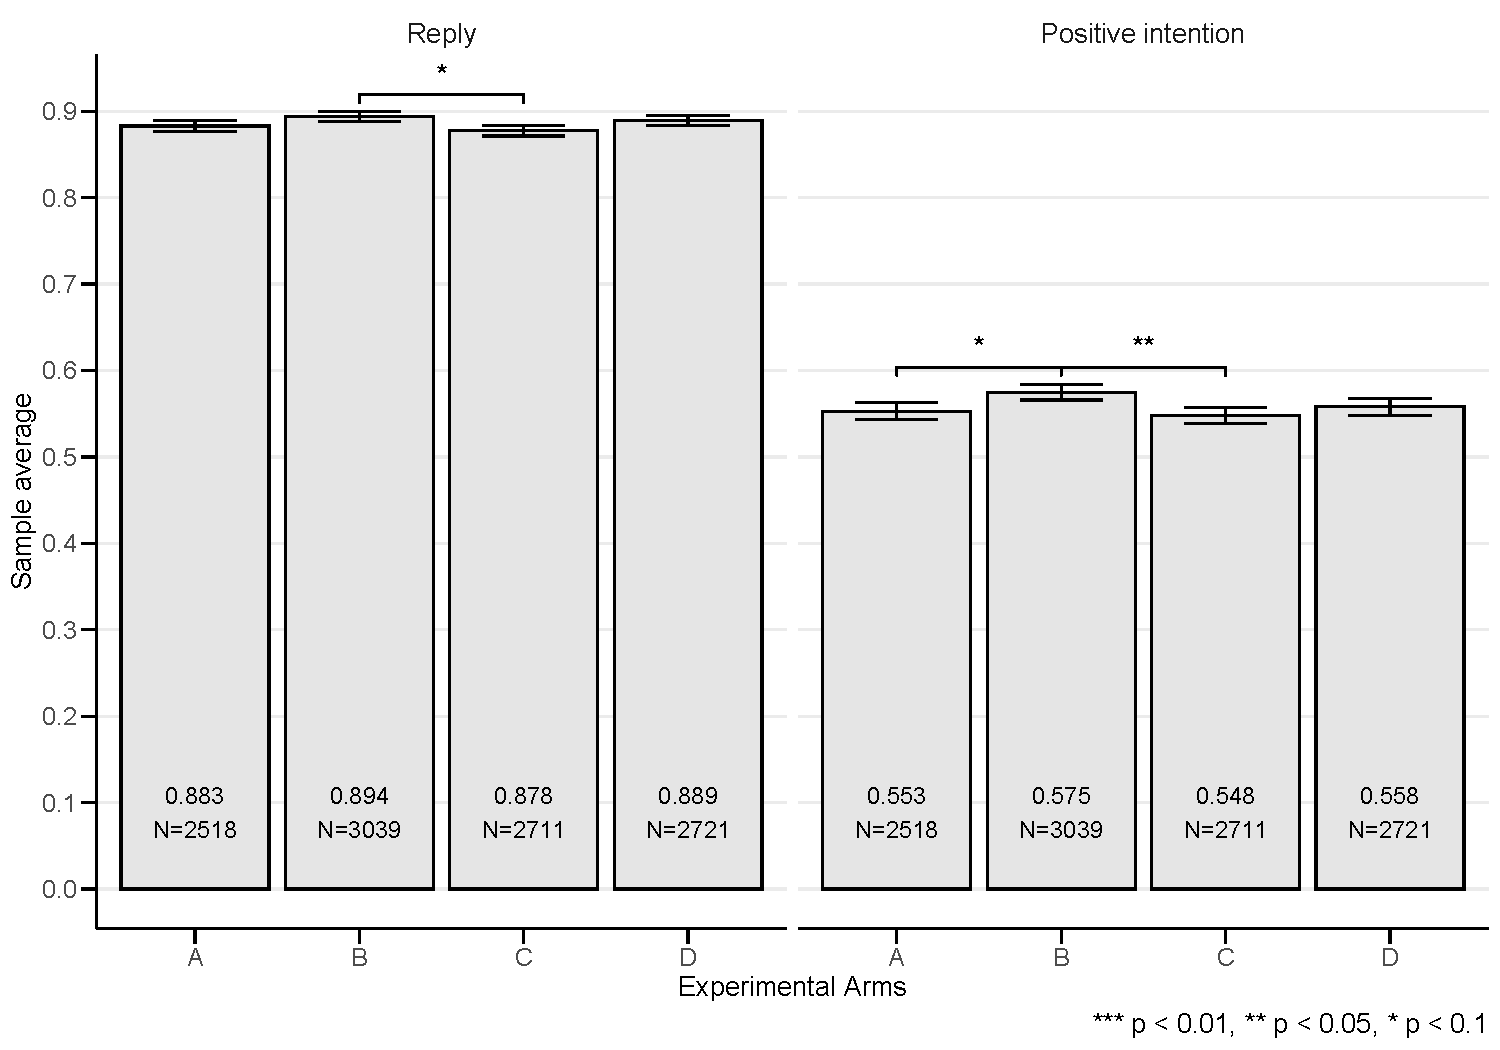
\includegraphics[width=0.75\linewidth]{C:/Users/vge00/Desktop/JMDP/RCT-Nudge/docs/slide/220826解析途中報告_files/figure-beamer/ttest-reply-1} \end{center}
\end{frame}

\begin{frame}{回帰分析の結果}
\protect\hypertarget{ux56deux5e30ux5206ux6790ux306eux7d50ux679c}{}
\begin{table}
\centering
\fontsize{8}{10}\selectfont
\begin{tabular}[t]{l>{\centering\arraybackslash}p{6em}>{\centering\arraybackslash}p{6em}>{\centering\arraybackslash}p{6em}>{\centering\arraybackslash}p{6em}>{\centering\arraybackslash}p{6em}}
\toprule
\multicolumn{2}{c}{ } & \multicolumn{4}{c}{Reply within specific day} \\
\cmidrule(l{3pt}r{3pt}){3-6}
\multicolumn{1}{c}{ } & \multicolumn{1}{c}{Reply} & \multicolumn{1}{c}{5 days} & \multicolumn{1}{c}{10 days} & \multicolumn{1}{c}{20 days} & \multicolumn{1}{c}{30 days} \\
\cmidrule(l{3pt}r{3pt}){2-2} \cmidrule(l{3pt}r{3pt}){3-3} \cmidrule(l{3pt}r{3pt}){4-4} \cmidrule(l{3pt}r{3pt}){5-5} \cmidrule(l{3pt}r{3pt}){6-6}
  & (1) & (2) & (3) & (4) & (5)\\
\midrule
B & \num{0.014}** & \num{0.005} & \num{-0.047}*** & \num{0.013} & \num{0.016}**\\
 & (\num{0.006}) & (\num{0.008}) & (\num{0.014}) & (\num{0.009}) & (\num{0.007})\\
C & \num{0.003} & \num{0.002} & \num{0.003} & \num{0.008} & \num{0.006}\\
 & (\num{0.005}) & (\num{0.007}) & (\num{0.015}) & (\num{0.007}) & (\num{0.005})\\
D & \num{0.006} & \num{0.013} & \num{-0.030}** & \num{0.017}** & \num{0.006}\\
 & (\num{0.005}) & (\num{0.009}) & (\num{0.014}) & (\num{0.007}) & (\num{0.005})\\
\midrule
Num.Obs. & \num{10989} & \num{10989} & \num{10989} & \num{10989} & \num{10989}\\
\addlinespace[0.3em]
\multicolumn{6}{l}{\textit{F-tests, p-value}}\\
\hspace{1em}B = C & \num{0.019} & \num{0.677} & \num{0.002} & \num{0.394} & \num{0.038}\\
\hspace{1em}B = D & \num{0.152} & \num{0.377} & \num{0.190} & \num{0.621} & \num{0.081}\\
\hspace{1em}C = D & \num{0.542} & \num{0.146} & \num{0.037} & \num{0.093} & \num{0.852}\\
\bottomrule
\multicolumn{6}{l}{\rule{0pt}{1em}* p $<$ 0.1, ** p $<$ 0.05, *** p $<$ 0.01}\\
\end{tabular}
\end{table}
\end{frame}

\begin{frame}{Remark:共変量・固定効果の影響}
\protect\hypertarget{remarkux5171ux5909ux91cfux56faux5b9aux52b9ux679cux306eux5f71ux97ff}{}
モデル(1)の共変量・固定効果に関する結果

\begin{itemize}
\tightlist
\item
  高齢であるほど、返信率が高い
\item
  女性の方が男性よりも返信率が高い
\item
  コーディネートの経験回数が多いほど、返信率が高い
\item
  東京・大阪・神奈川・愛知に在住している人がそうでない人よりも返信率が高い
\item
  週・月の固定効果は返信率と\textbf{相関なし}
\end{itemize}
\end{frame}

\begin{frame}{回帰分析と二群比較の結果の差について(メモ)}
\protect\hypertarget{ux56deux5e30ux5206ux6790ux3068ux4e8cux7fa4ux6bd4ux8f03ux306eux7d50ux679cux306eux5deeux306bux3064ux3044ux3066ux30e1ux30e2}{}
メッセージAとメッセージBの比較に注目する

\begin{itemize}
\tightlist
\item
  効果の大きさ:0.011(二群比較)\(<\) 0.014(回帰分析)

  \begin{itemize}
  \tightlist
  \item
    回帰分析はA群の平均年齢と平均コーディネート経験回数がB群よりも若干高いことを制御した?
  \end{itemize}
\item
  推定効果の標準誤差:0.009(二群比較)\(>\) 0.006(回帰分析)

  \begin{itemize}
  \tightlist
  \item
    回帰分析は実験週単位でクラスターした標準誤差を使用している
  \item
    クラスター標準誤差が通常の標準誤差を下回るということは、
    クラスター内の個人間の相関が負であることを示す (Angrist and Pischke, 2009)
  \item
    適合通知を受け取った人が他の人の返信状況などを聞いて、
    クラウディング・アウトのような行動を取るとしたら、クラスター内の個人間の相関が負となる?
  \end{itemize}
\end{itemize}
\end{frame}

\begin{frame}{移植の意向による効果の分解}
\protect\hypertarget{ux79fbux690dux306eux610fux5411ux306bux3088ux308bux52b9ux679cux306eux5206ux89e3}{}
\begin{itemize}
\tightlist
\item
  返信率に対する効果は2つの効果に分解できる

  \begin{enumerate}
  \tightlist
  \item
    \textbf{Positive intention}:提供を希望して返信したかどうか
  \item
    \textbf{Negative intention}:提供を希望しないで返信したかどうか
  \end{enumerate}
\item
  意向に関する二つのアウトカム変数に対する効果を推定する
\item
  また、返信スピードを考慮して、
  \(X\)日以内に提供を希望して(しないで)返信したかどうかもアウトカム
  (Reply within specific day with psotive/negative intention)としたモデルも推定する
\end{itemize}
\end{frame}

\begin{frame}{Positive intentionに対する効果}
\protect\hypertarget{positive-intentionux306bux5bfeux3059ux308bux52b9ux679c}{}
\begin{table}
\centering
\fontsize{8}{10}\selectfont
\begin{tabular}[t]{l>{\centering\arraybackslash}p{6em}>{\centering\arraybackslash}p{6em}>{\centering\arraybackslash}p{6em}>{\centering\arraybackslash}p{6em}>{\centering\arraybackslash}p{6em}}
\toprule
\multicolumn{2}{c}{ } & \multicolumn{4}{c}{Reply within specific day with positive intention} \\
\cmidrule(l{3pt}r{3pt}){3-6}
\multicolumn{1}{c}{ } & \multicolumn{1}{c}{Positive intention} & \multicolumn{1}{c}{5 days} & \multicolumn{1}{c}{10 days} & \multicolumn{1}{c}{20 days} & \multicolumn{1}{c}{30 days} \\
\cmidrule(l{3pt}r{3pt}){2-2} \cmidrule(l{3pt}r{3pt}){3-3} \cmidrule(l{3pt}r{3pt}){4-4} \cmidrule(l{3pt}r{3pt}){5-5} \cmidrule(l{3pt}r{3pt}){6-6}
  & (1) & (2) & (3) & (4) & (5)\\
\midrule
B & \num{0.020} & \num{0.013} & \num{-0.020}* & \num{0.021} & \num{0.021}\\
 & (\num{0.012}) & (\num{0.009}) & (\num{0.010}) & (\num{0.013}) & (\num{0.012})\\
C & \num{-0.003} & \num{0.004} & \num{0.005} & \num{-0.002} & \num{-0.003}\\
 & (\num{0.011}) & (\num{0.009}) & (\num{0.015}) & (\num{0.011}) & (\num{0.011})\\
D & \num{0.006} & \num{0.016} & \num{-0.016} & \num{0.013} & \num{0.007}\\
 & (\num{0.010}) & (\num{0.010}) & (\num{0.011}) & (\num{0.011}) & (\num{0.010})\\
\midrule
Num.Obs. & \num{10989} & \num{10989} & \num{10989} & \num{10989} & \num{10989}\\
\addlinespace[0.3em]
\multicolumn{6}{l}{\textit{F-tests, p-value}}\\
\hspace{1em}B = C & \num{0.011} & \num{0.227} & \num{0.087} & \num{0.014} & \num{0.007}\\
\hspace{1em}B = D & \num{0.071} & \num{0.775} & \num{0.691} & \num{0.395} & \num{0.078}\\
\hspace{1em}C = D & \num{0.256} & \num{0.145} & \num{0.122} & \num{0.037} & \num{0.149}\\
\bottomrule
\multicolumn{6}{l}{\rule{0pt}{1em}* p $<$ 0.1, ** p $<$ 0.05, *** p $<$ 0.01}\\
\end{tabular}
\end{table}
\end{frame}

\begin{frame}{Remark:共変量・固定効果の影響}
\protect\hypertarget{remarkux5171ux5909ux91cfux56faux5b9aux52b9ux679cux306eux5f71ux97ff-1}{}
モデル(1)の共変量・固定効果に関する結果

\begin{itemize}
\tightlist
\item
  高齢であるほど、正の意向を示しやすい
\item
  男性の方が女性よりも正の意向を示しやすい
\item
  コーディネートの経験回数が多いほど、正の意向を示さない
\item
  2022年1月と比較して、2021/9や2021/10に送付した時の方が正の意向を示しやすい
\item
  第1週と比較して、第3週に送付したときの方が正の意向を示しやすい
\end{itemize}
\end{frame}

\begin{frame}{回帰分析と二群比較の結果の差について(メモ)}
\protect\hypertarget{ux56deux5e30ux5206ux6790ux3068ux4e8cux7fa4ux6bd4ux8f03ux306eux7d50ux679cux306eux5deeux306bux3064ux3044ux3066ux30e1ux30e2-1}{}
メッセージAとメッセージBの比較に注目する

\begin{itemize}
\tightlist
\item
  効果の大きさ:0.022(二群比較)\(>\) 0.020(回帰分析)

  \begin{itemize}
  \tightlist
  \item
    回帰分析はA群の平均年齢と平均コーディネート経験回数がB群よりも若干高いことを制御した?
  \item
    メッセージBの割り当ては第1週に2回、第3週に1回。
    メッセージAの割り当ては第1週と第3週ともに1回。
  \end{itemize}
\item
  推定効果の標準誤差:0.013(二群比較)\(>\) 0.012(回帰分析)

  \begin{itemize}
  \tightlist
  \item
    回帰分析は実験週単位でクラスターした標準誤差を使用している
  \item
    クラスター標準誤差が通常の標準誤差を下回るということは、
    クラスター内の個人間の相関が負であることを示す
  \end{itemize}
\end{itemize}
\end{frame}

\begin{frame}{Negative intentionに対する効果}
\protect\hypertarget{negative-intentionux306bux5bfeux3059ux308bux52b9ux679c}{}
\begin{table}
\centering
\fontsize{8}{10}\selectfont
\begin{tabular}[t]{l>{\centering\arraybackslash}p{6em}>{\centering\arraybackslash}p{6em}>{\centering\arraybackslash}p{6em}>{\centering\arraybackslash}p{6em}>{\centering\arraybackslash}p{6em}}
\toprule
\multicolumn{2}{c}{ } & \multicolumn{4}{c}{Reply within specific day with negative intention} \\
\cmidrule(l{3pt}r{3pt}){3-6}
\multicolumn{1}{c}{ } & \multicolumn{1}{c}{Negative intention} & \multicolumn{1}{c}{5 days} & \multicolumn{1}{c}{10 days} & \multicolumn{1}{c}{20 days} & \multicolumn{1}{c}{30 days} \\
\cmidrule(l{3pt}r{3pt}){2-2} \cmidrule(l{3pt}r{3pt}){3-3} \cmidrule(l{3pt}r{3pt}){4-4} \cmidrule(l{3pt}r{3pt}){5-5} \cmidrule(l{3pt}r{3pt}){6-6}
  & (1) & (2) & (3) & (4) & (5)\\
\midrule
B & \num{-0.006} & \num{-0.008}* & \num{-0.028}*** & \num{-0.008} & \num{-0.005}\\
 & (\num{0.008}) & (\num{0.005}) & (\num{0.008}) & (\num{0.007}) & (\num{0.007})\\
C & \num{0.006} & \num{-0.002} & \num{-0.002} & \num{0.010} & \num{0.009}\\
 & (\num{0.010}) & (\num{0.005}) & (\num{0.009}) & (\num{0.007}) & (\num{0.009})\\
D & \num{0.000} & \num{-0.003} & \num{-0.013}* & \num{0.003} & \num{-0.001}\\
 & (\num{0.007}) & (\num{0.005}) & (\num{0.007}) & (\num{0.007}) & (\num{0.007})\\
\midrule
Num.Obs. & \num{10989} & \num{10989} & \num{10989} & \num{10989} & \num{10989}\\
\addlinespace[0.3em]
\multicolumn{6}{l}{\textit{F-tests, p-value}}\\
\hspace{1em}B = C & \num{0.159} & \num{0.114} & \num{0.014} & \num{0.008} & \num{0.079}\\
\hspace{1em}B = D & \num{0.190} & \num{0.138} & \num{0.117} & \num{0.060} & \num{0.381}\\
\hspace{1em}C = D & \num{0.452} & \num{0.822} & \num{0.256} & \num{0.302} & \num{0.194}\\
\bottomrule
\multicolumn{6}{l}{\rule{0pt}{1em}* p $<$ 0.1, ** p $<$ 0.05, *** p $<$ 0.01}\\
\end{tabular}
\end{table}
\end{frame}

\begin{frame}{性別×年齢による効果の異質性}
\protect\hypertarget{ux6027ux5225ux5e74ux9f62ux306bux3088ux308bux52b9ux679cux306eux7570ux8ceaux6027}{}
\begin{itemize}
\tightlist
\item
  性別と年齢(30歳以下どうか)でサンプルを分割して、返信と意向の効果を推定する

  \begin{itemize}
  \tightlist
  \item
    \textbf{若年男性は移植実績が良いとされているが、具体的に、若年とは何歳以下か?}
  \end{itemize}
\end{itemize}
\end{frame}

\begin{frame}{性別×年齢による効果の異質性:結果(1)}
\protect\hypertarget{ux6027ux5225ux5e74ux9f62ux306bux3088ux308bux52b9ux679cux306eux7570ux8ceaux6027ux7d50ux679c1}{}
\begin{center}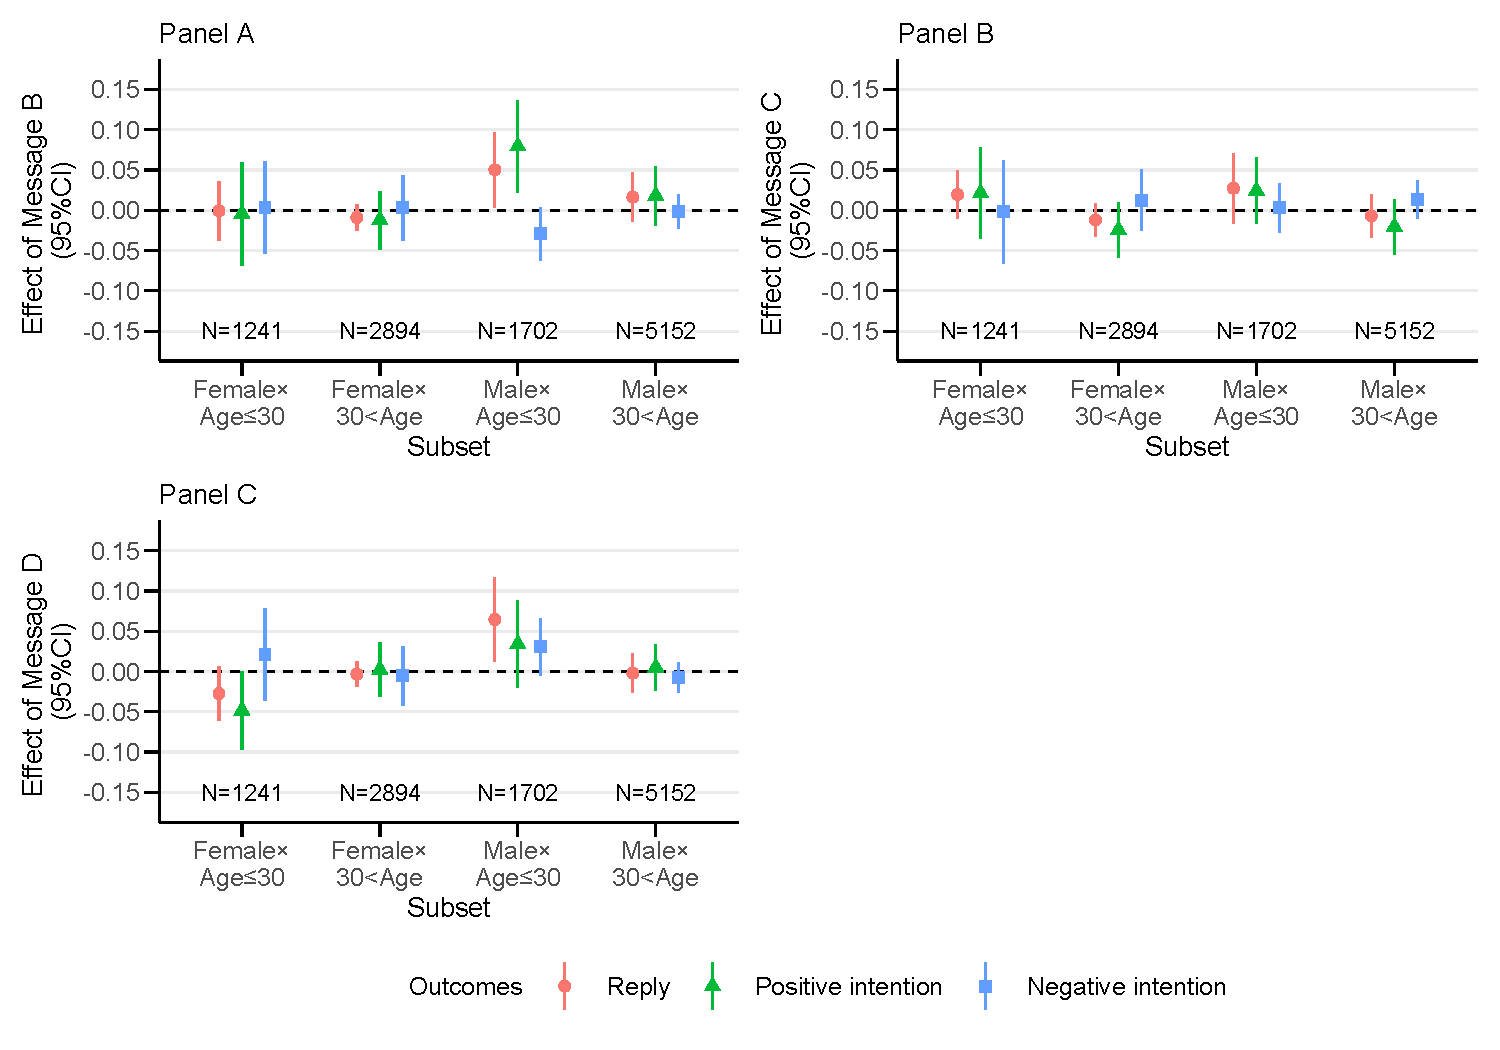
\includegraphics[width=0.75\linewidth]{C:/Users/vge00/Desktop/JMDP/RCT-Nudge/docs/slide/220826解析途中報告_files/figure-beamer/plot-hetero-reply-gender-age-1} \end{center}
\end{frame}

\begin{frame}{性別×年齢による効果の異質性:結果(2)}
\protect\hypertarget{ux6027ux5225ux5e74ux9f62ux306bux3088ux308bux52b9ux679cux306eux7570ux8ceaux6027ux7d50ux679c2}{}
\begin{center}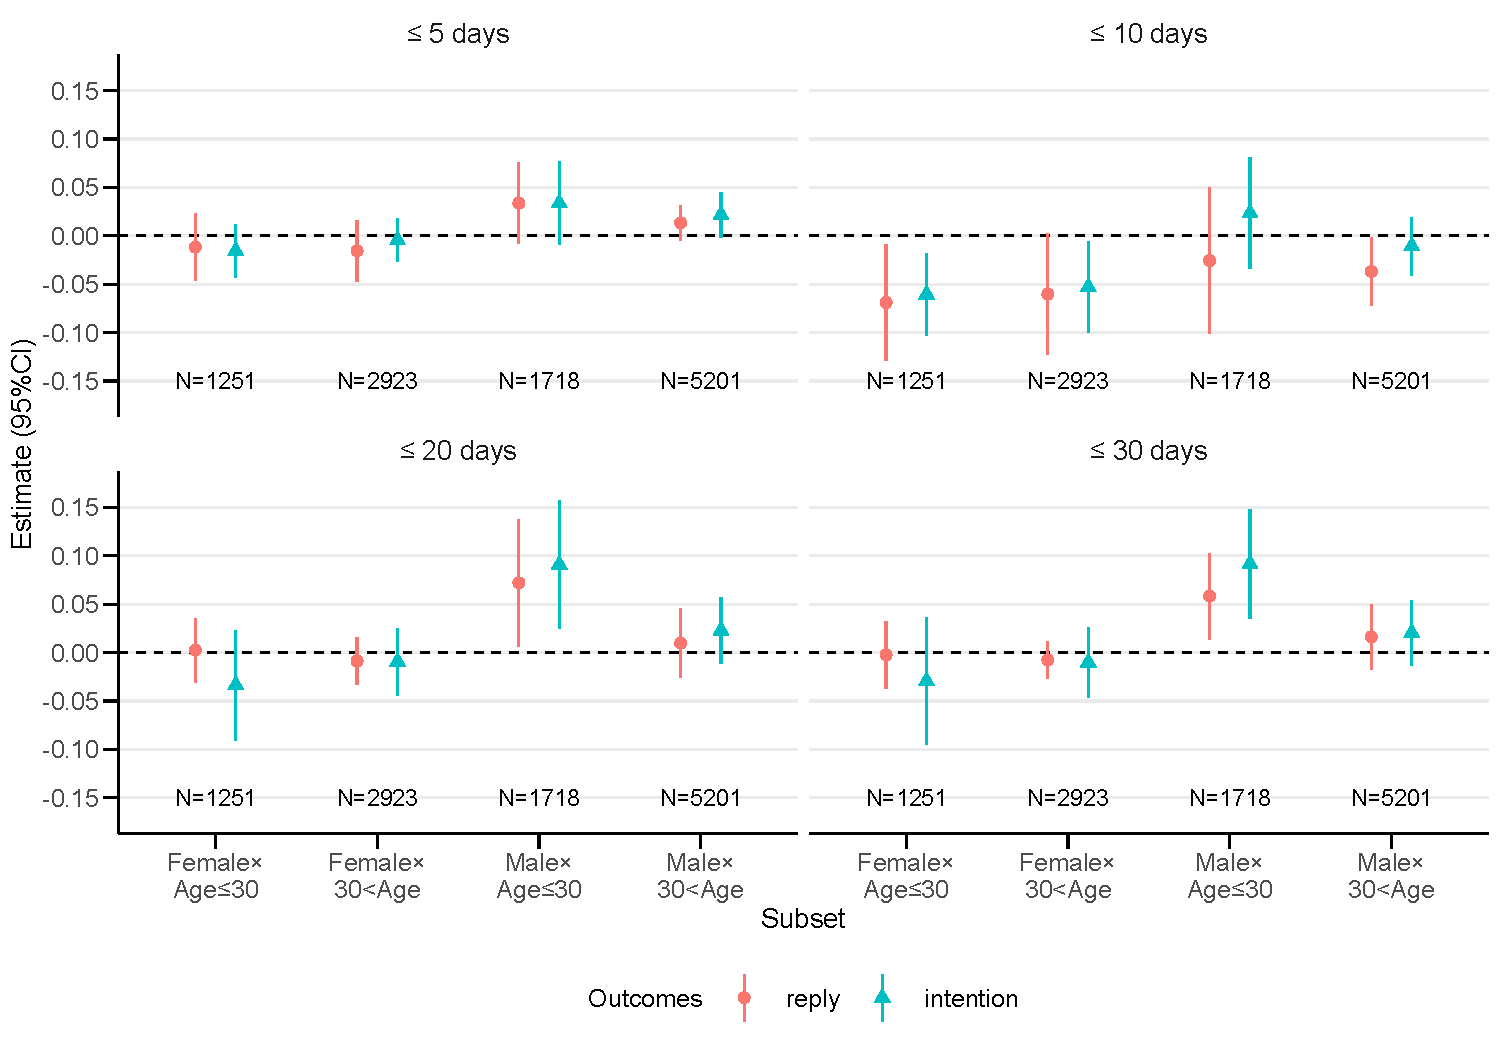
\includegraphics[width=0.75\linewidth]{C:/Users/vge00/Desktop/JMDP/RCT-Nudge/docs/slide/220826解析途中報告_files/figure-beamer/plotB-hetero-reply-within-gender-age-1} \end{center}
\end{frame}

\begin{frame}{性別×年齢による効果の異質性:結果(3)}
\protect\hypertarget{ux6027ux5225ux5e74ux9f62ux306bux3088ux308bux52b9ux679cux306eux7570ux8ceaux6027ux7d50ux679c3}{}
\begin{center}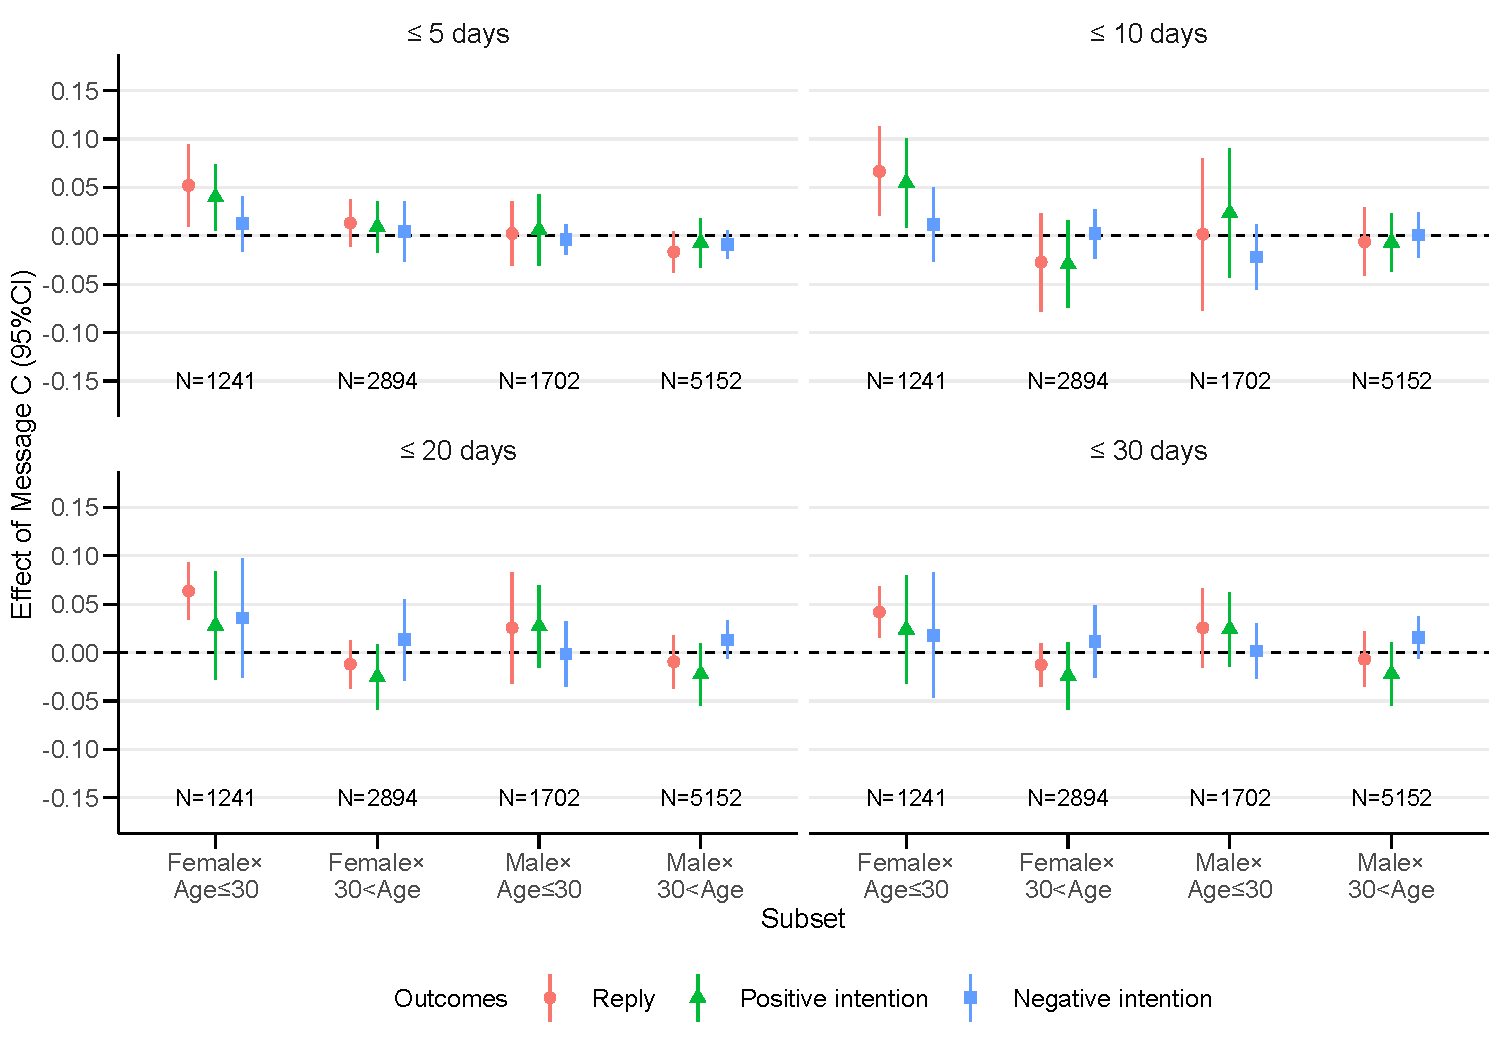
\includegraphics[width=0.75\linewidth]{C:/Users/vge00/Desktop/JMDP/RCT-Nudge/docs/slide/220826解析途中報告_files/figure-beamer/plotC-hetero-reply-within-gender-age-1} \end{center}
\end{frame}

\begin{frame}{性別×年齢による効果の異質性:結果(4)}
\protect\hypertarget{ux6027ux5225ux5e74ux9f62ux306bux3088ux308bux52b9ux679cux306eux7570ux8ceaux6027ux7d50ux679c4}{}
\begin{center}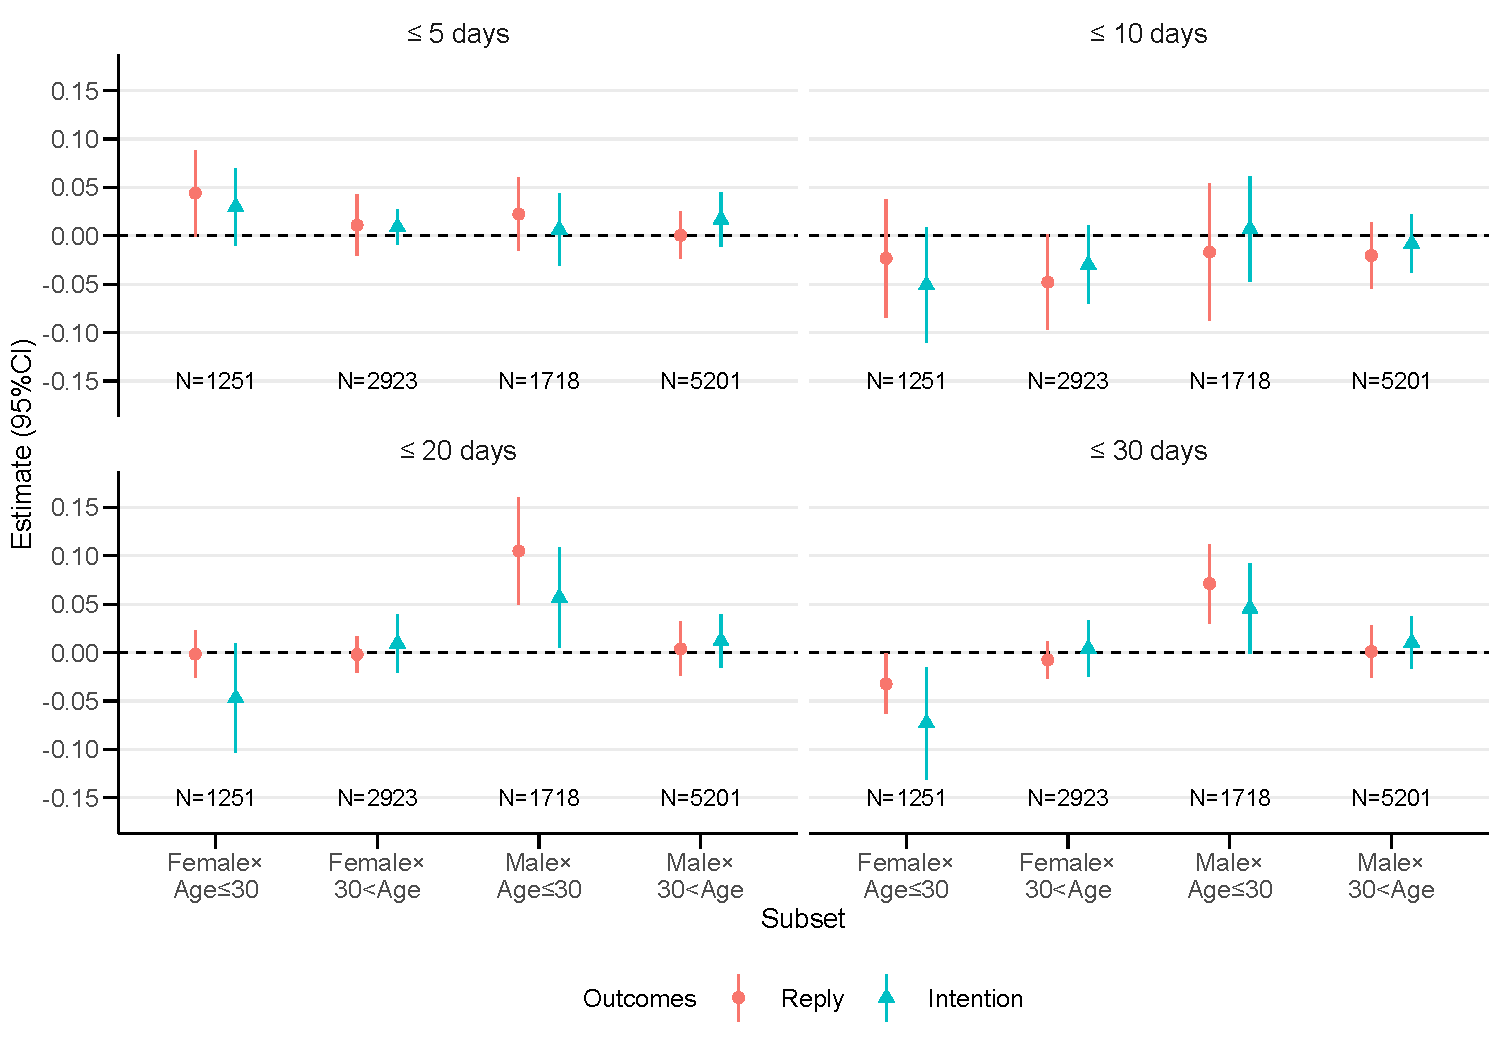
\includegraphics[width=0.75\linewidth]{C:/Users/vge00/Desktop/JMDP/RCT-Nudge/docs/slide/220826解析途中報告_files/figure-beamer/plotD-hetero-reply-within-gender-age-1} \end{center}
\end{frame}

\begin{frame}{地域による異質性}
\protect\hypertarget{ux5730ux57dfux306bux3088ux308bux7570ux8ceaux6027}{}
\begin{itemize}
\tightlist
\item
  都道府県ごとに10平方キロメートル当たりの病院数を計算し、
  0.5カ所以上ある地域とそうでない地域でサンプルを分割した

  \begin{itemize}
  \tightlist
  \item
    1カ所以上:東京・大阪
  \item
    1カ所未満:神奈川・愛知
  \item
    東京・大阪・神奈川・愛知のグループを\emph{TOKA}と称する
  \end{itemize}
\item
  それぞれのサブサンプルで効果を推定する。さらに、性別×TOKAのサブサンプルでも効果を推定する。
\end{itemize}
\end{frame}

\begin{frame}{地域による効果の異質性(1)}
\protect\hypertarget{ux5730ux57dfux306bux3088ux308bux52b9ux679cux306eux7570ux8ceaux60271}{}
\begin{center}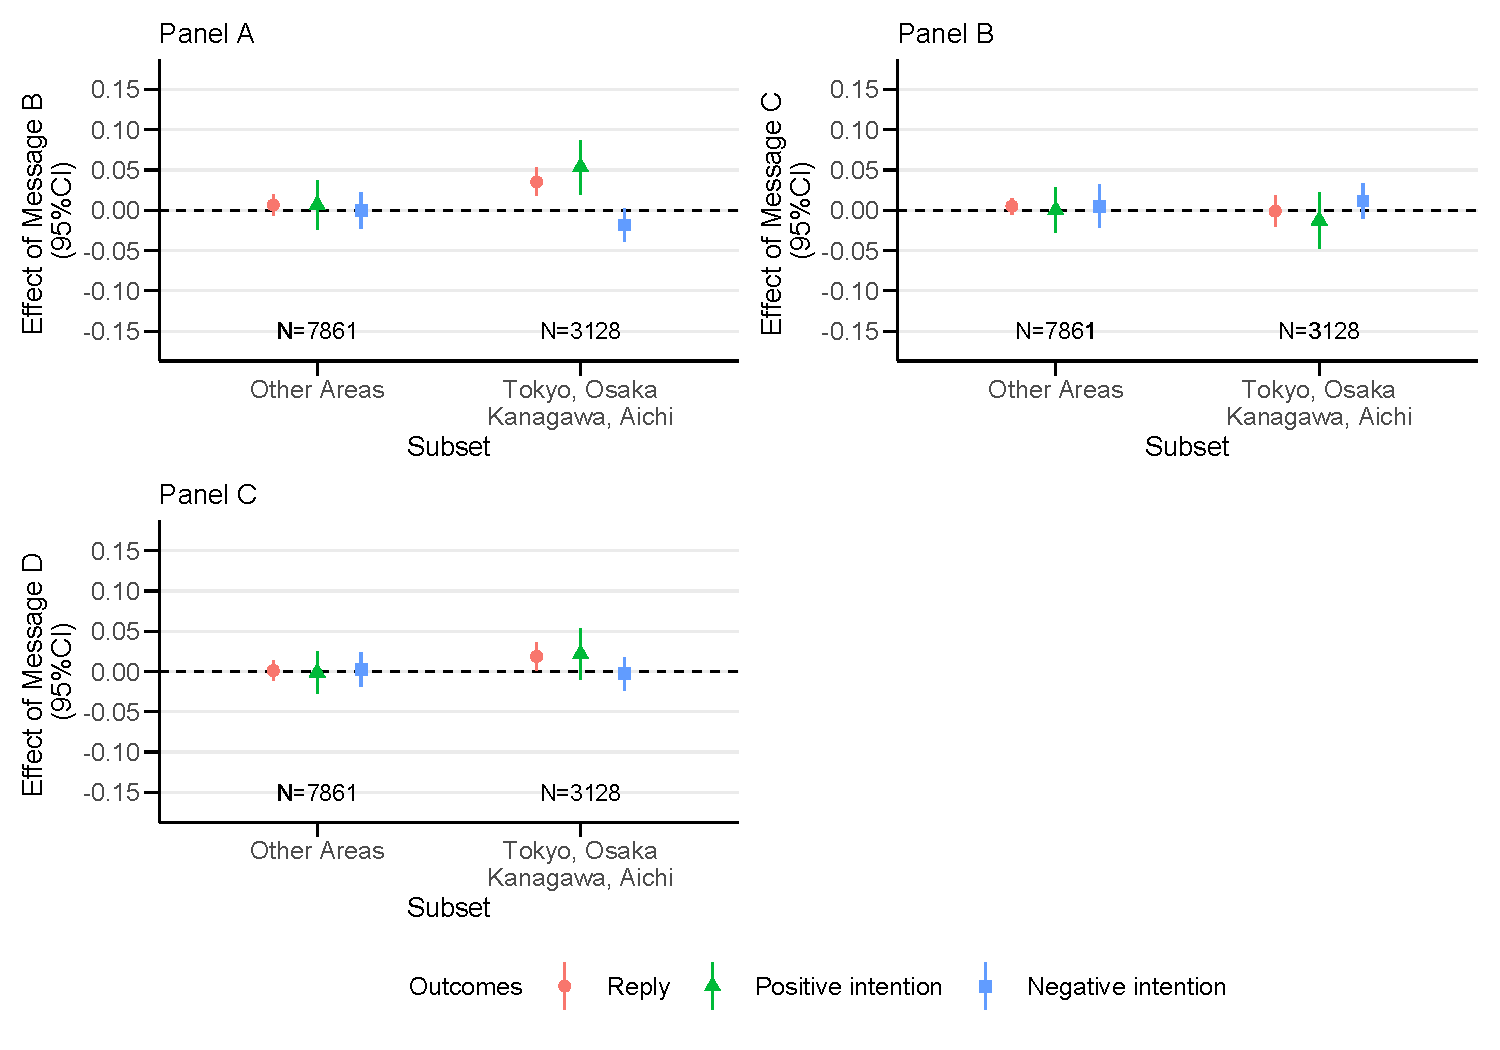
\includegraphics[width=0.75\linewidth]{C:/Users/vge00/Desktop/JMDP/RCT-Nudge/docs/slide/220826解析途中報告_files/figure-beamer/plotB-hetero-reply-geo-1} \end{center}
\end{frame}

\begin{frame}{地域による効果の異質性(2)}
\protect\hypertarget{ux5730ux57dfux306bux3088ux308bux52b9ux679cux306eux7570ux8ceaux60272}{}
\begin{center}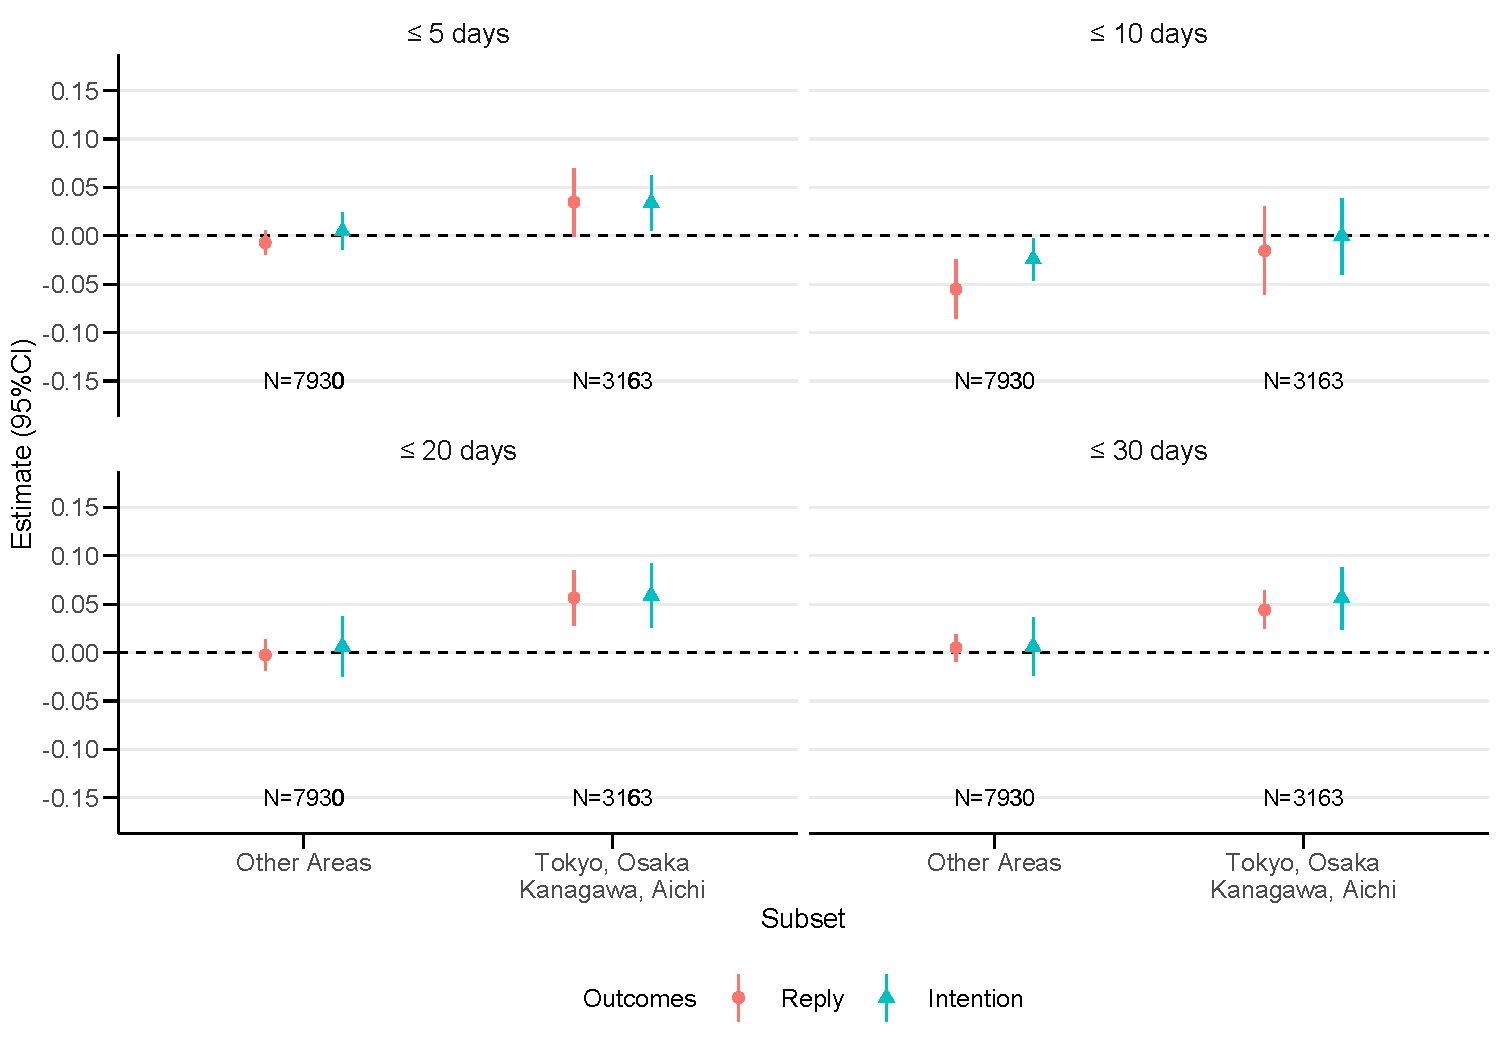
\includegraphics[width=0.75\linewidth]{C:/Users/vge00/Desktop/JMDP/RCT-Nudge/docs/slide/220826解析途中報告_files/figure-beamer/plotB-hetero-reply-within-geo-1} \end{center}
\end{frame}

\begin{frame}{地域による効果の異質性(3)}
\protect\hypertarget{ux5730ux57dfux306bux3088ux308bux52b9ux679cux306eux7570ux8ceaux60273}{}
\begin{center}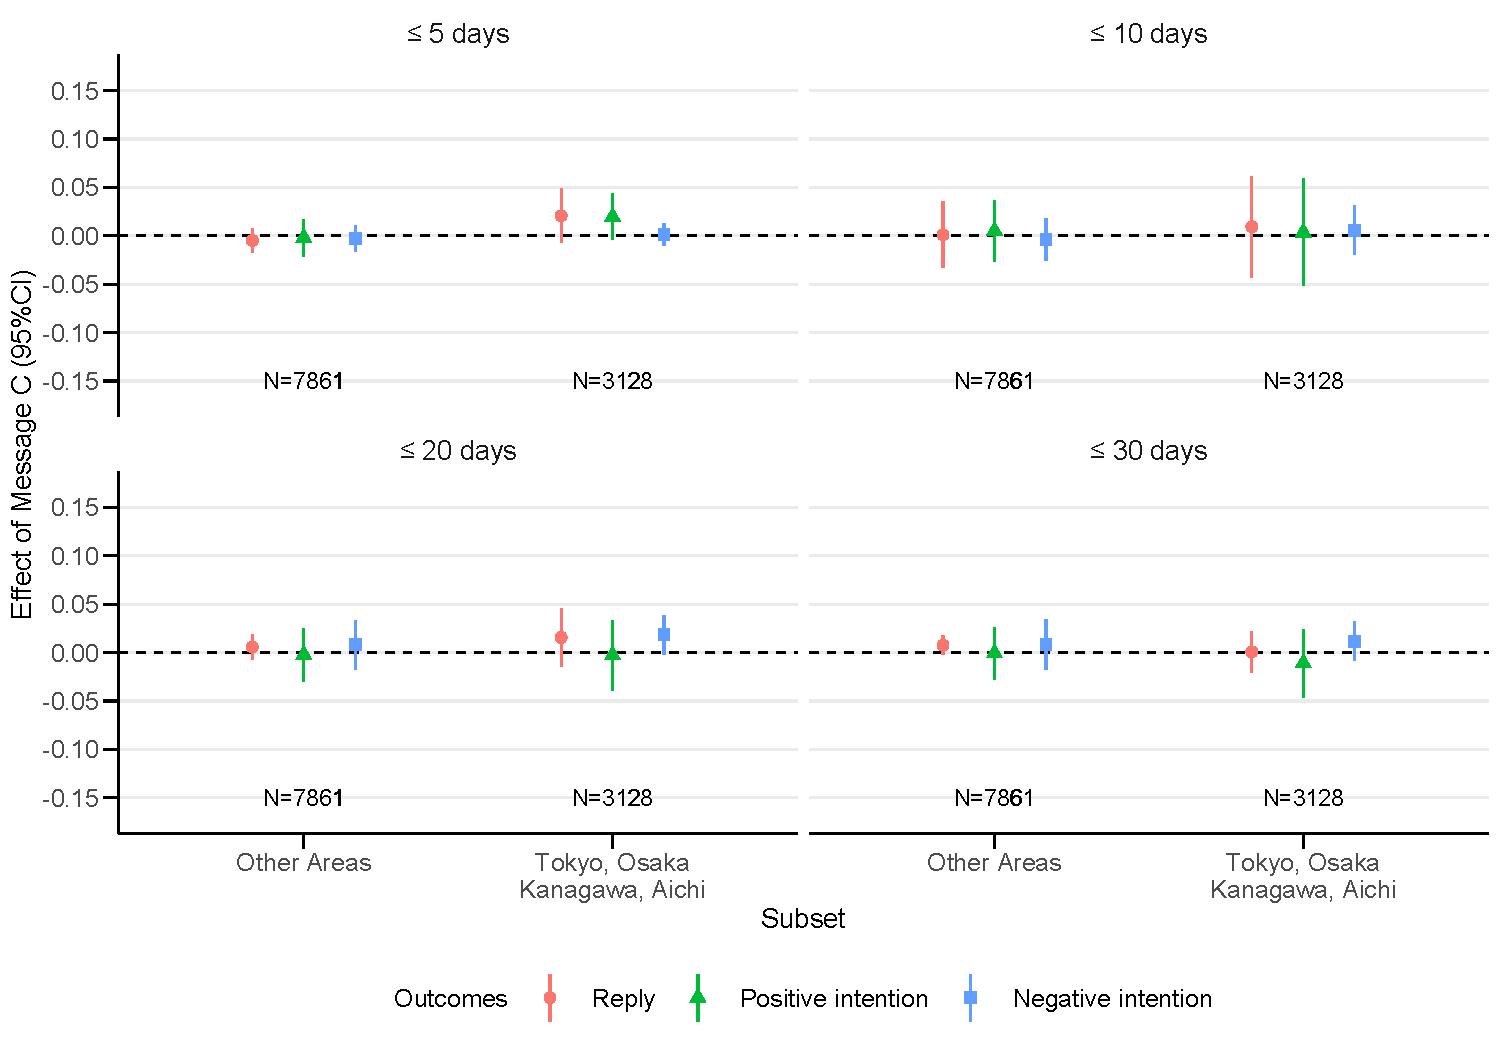
\includegraphics[width=0.75\linewidth]{C:/Users/vge00/Desktop/JMDP/RCT-Nudge/docs/slide/220826解析途中報告_files/figure-beamer/plotC-hetero-reply-within-geo-1} \end{center}
\end{frame}

\begin{frame}{地域による効果の異質性(4)}
\protect\hypertarget{ux5730ux57dfux306bux3088ux308bux52b9ux679cux306eux7570ux8ceaux60274}{}
\begin{center}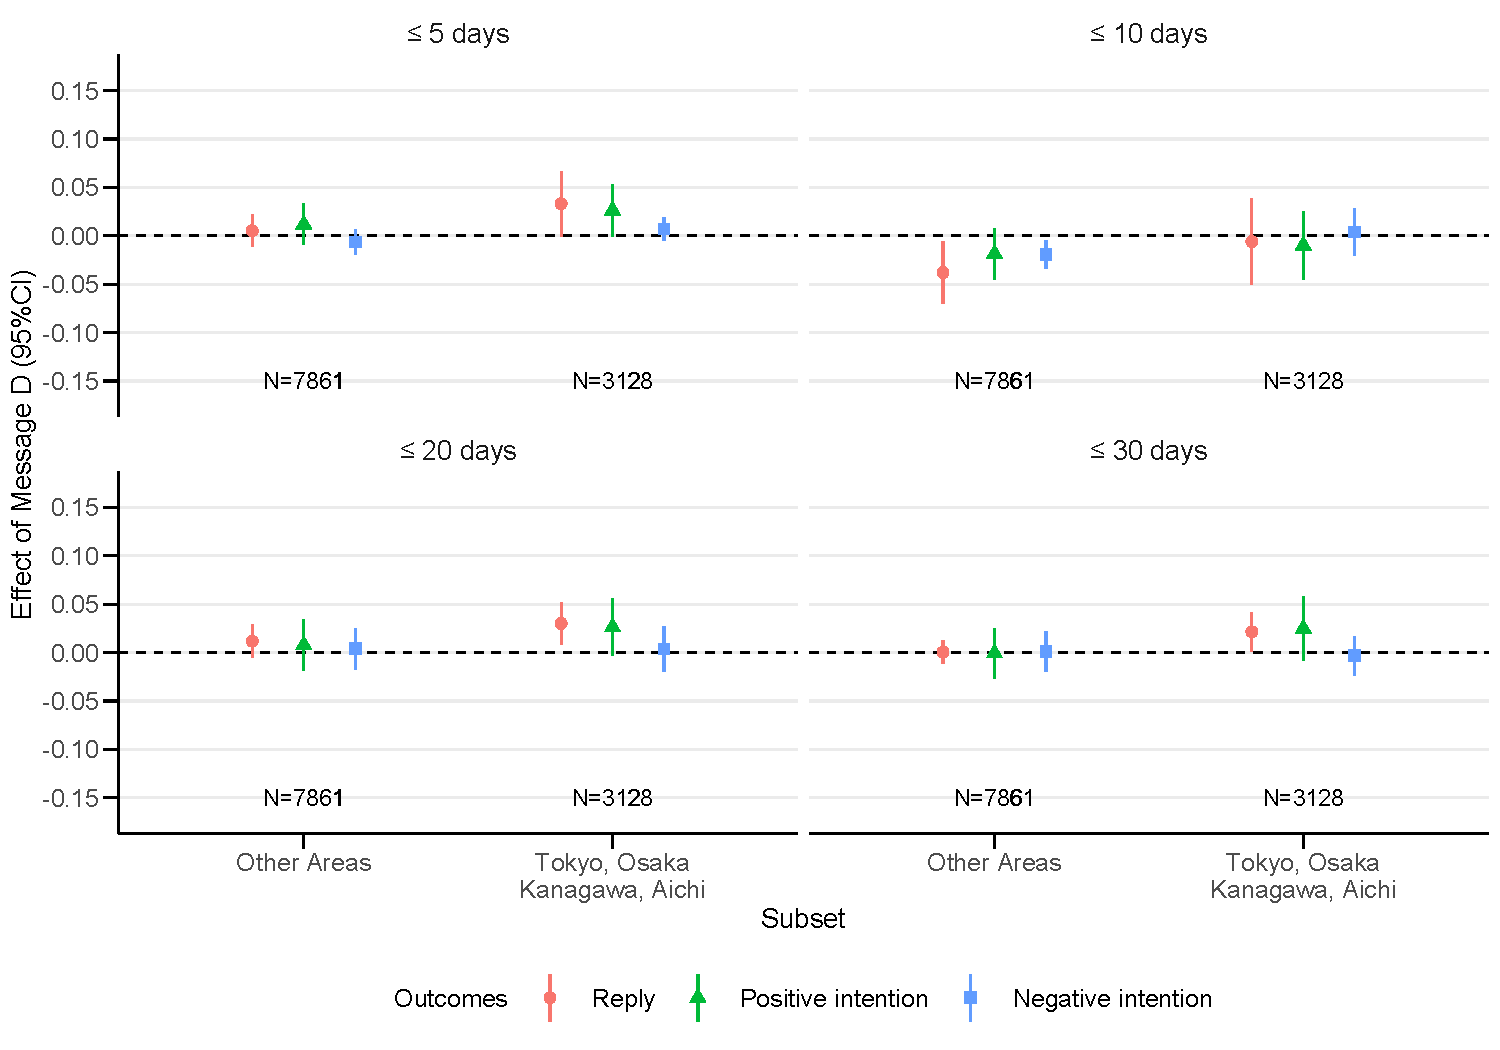
\includegraphics[width=0.75\linewidth]{C:/Users/vge00/Desktop/JMDP/RCT-Nudge/docs/slide/220826解析途中報告_files/figure-beamer/plotD-hetero-reply-within-geo-1} \end{center}
\end{frame}

\begin{frame}{性別×TOKA地域による効果の異質性(1)}
\protect\hypertarget{ux6027ux5225tokaux5730ux57dfux306bux3088ux308bux52b9ux679cux306eux7570ux8ceaux60271}{}
\begin{center}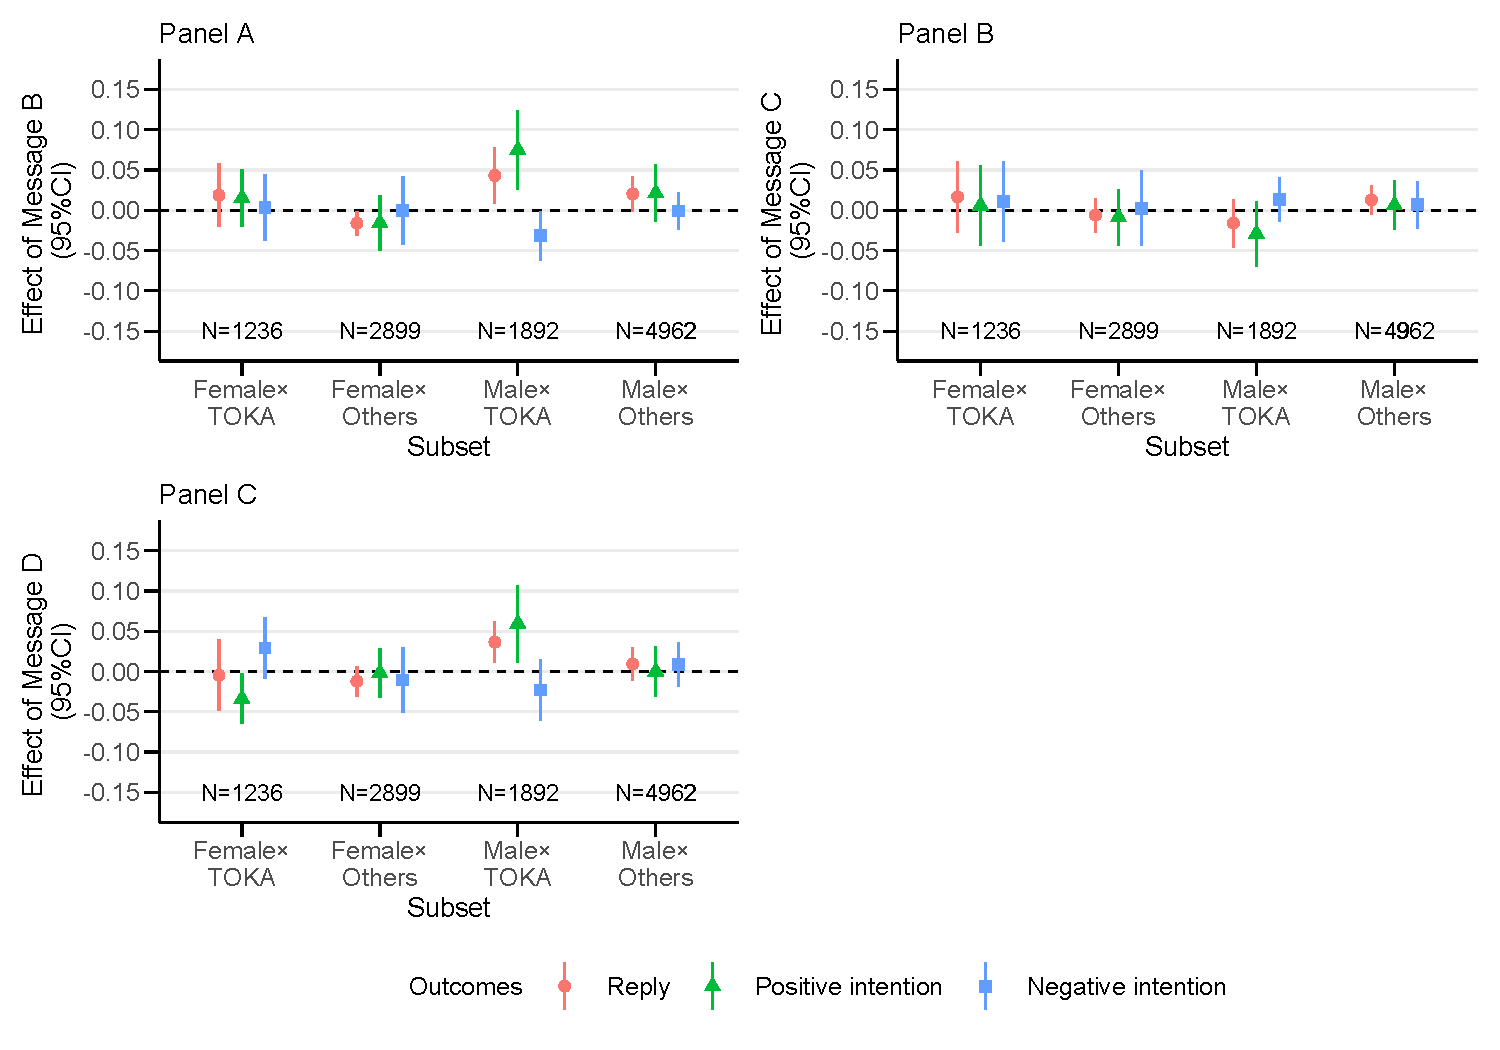
\includegraphics[width=0.75\linewidth]{C:/Users/vge00/Desktop/JMDP/RCT-Nudge/docs/slide/220826解析途中報告_files/figure-beamer/plotB-hetero-reply-gender-geo-1} \end{center}
\end{frame}

\begin{frame}{性別×TOKA地域による効果の異質性(2)}
\protect\hypertarget{ux6027ux5225tokaux5730ux57dfux306bux3088ux308bux52b9ux679cux306eux7570ux8ceaux60272}{}
\begin{center}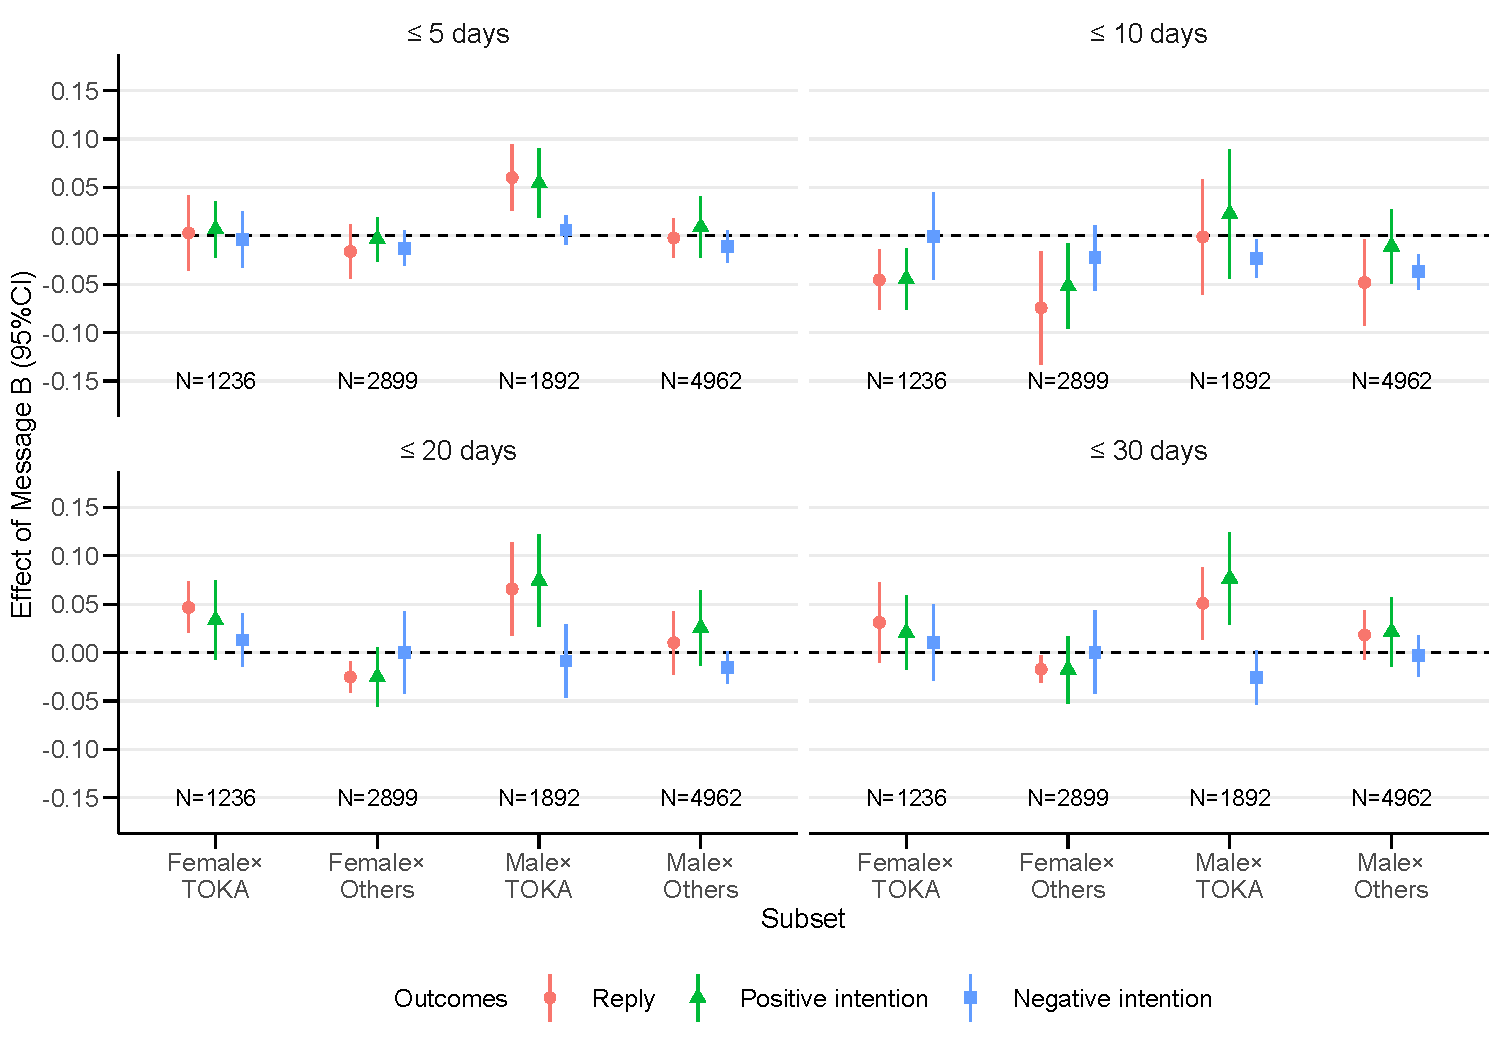
\includegraphics[width=0.75\linewidth]{C:/Users/vge00/Desktop/JMDP/RCT-Nudge/docs/slide/220826解析途中報告_files/figure-beamer/plotB-hetero-reply-within-gender-geo-1} \end{center}
\end{frame}

\begin{frame}{性別×TOKA地域による効果の異質性(3)}
\protect\hypertarget{ux6027ux5225tokaux5730ux57dfux306bux3088ux308bux52b9ux679cux306eux7570ux8ceaux60273}{}
\begin{center}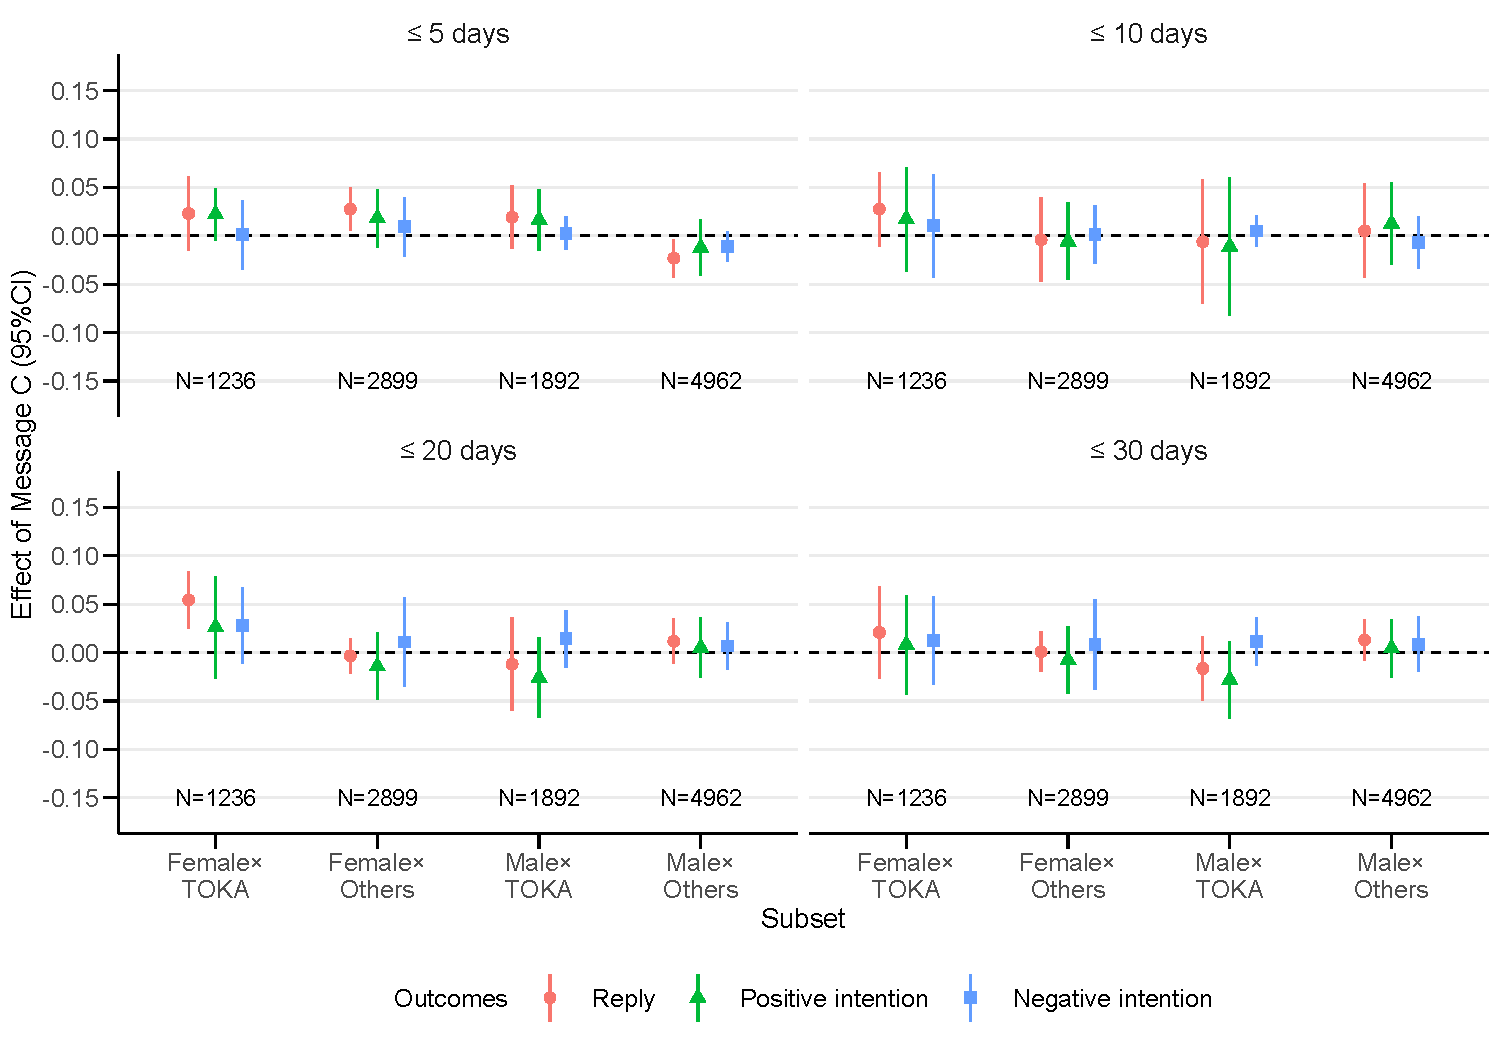
\includegraphics[width=0.75\linewidth]{C:/Users/vge00/Desktop/JMDP/RCT-Nudge/docs/slide/220826解析途中報告_files/figure-beamer/plotC-hetero-reply-within-gender-geo-1} \end{center}
\end{frame}

\begin{frame}{性別×TOKA地域による効果の異質性(4)}
\protect\hypertarget{ux6027ux5225tokaux5730ux57dfux306bux3088ux308bux52b9ux679cux306eux7570ux8ceaux60274}{}
\begin{center}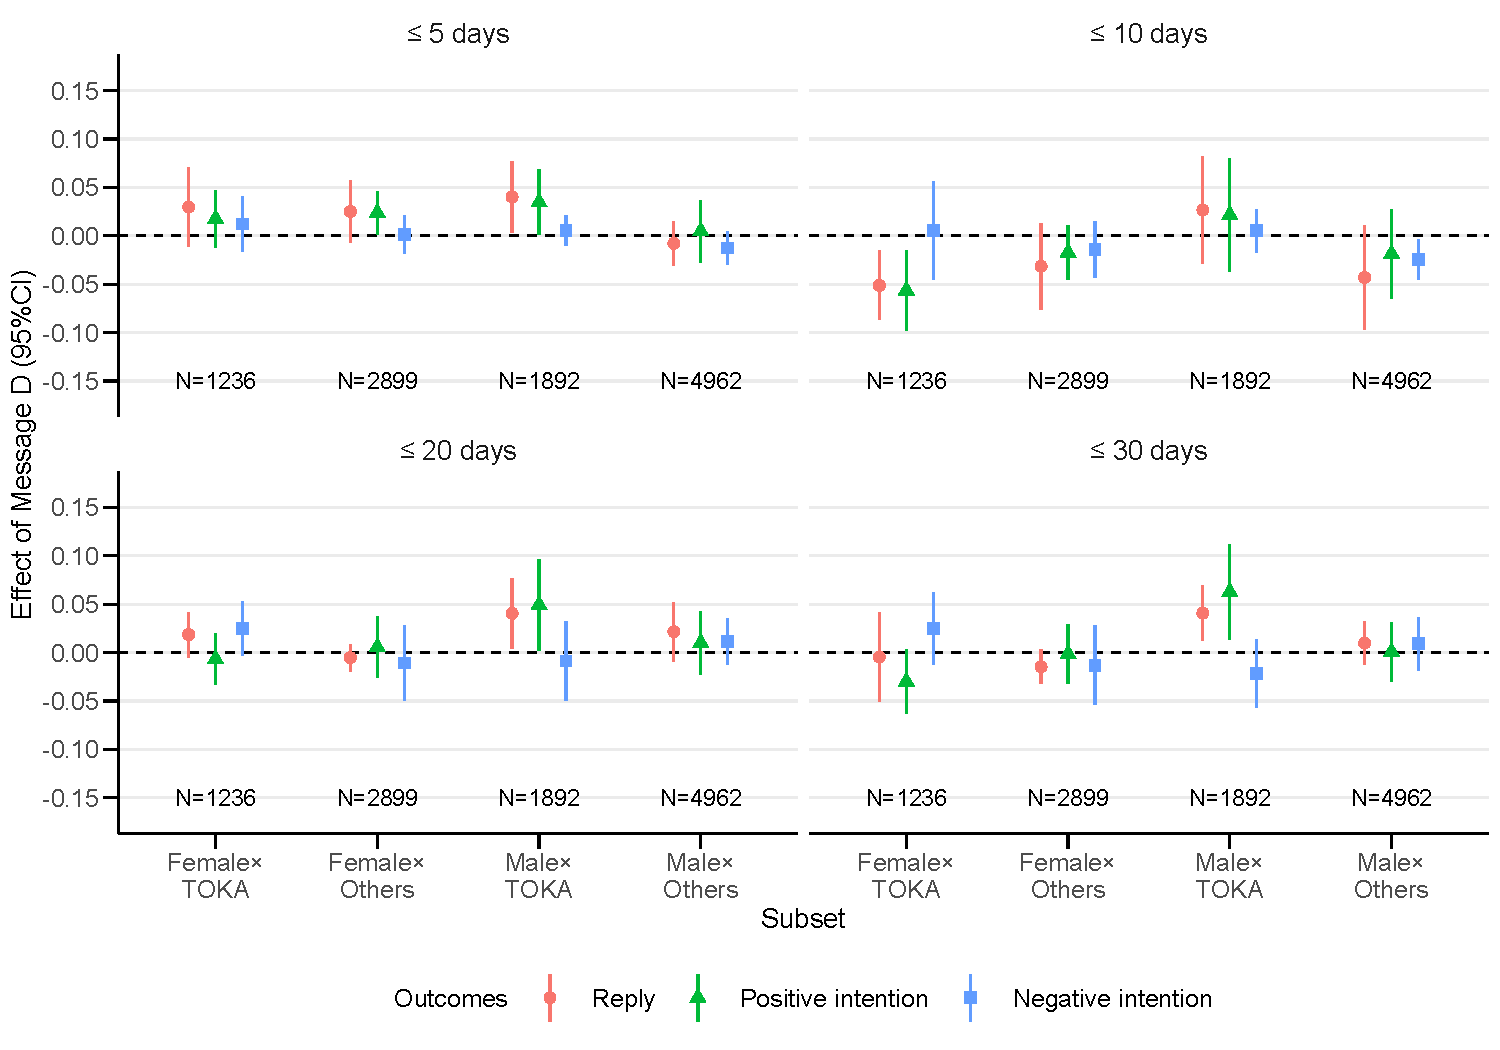
\includegraphics[width=0.75\linewidth]{C:/Users/vge00/Desktop/JMDP/RCT-Nudge/docs/slide/220826解析途中報告_files/figure-beamer/plotD-hetero-reply-within-gender-geo-1} \end{center}
\end{frame}

\end{document}
